\chapter{Estereoquímica: quiralidad e isómeros}\label{ch:g12:stereochemistry}

Las hojas de hierbabuena y las semillas de alcaravea no huelen en
absoluto igual: una tiene el olor fresco del chicle, la otra el olor
cálido del pan de centeno. Sin embargo, la \omterm{def:g7:atoms-and-molecules:molecule}{molécula} responsable de cada
olor es la misma carvona, formada por los mismos \omterm{def:g7:atoms-and-molecules:atom}{átomos} unidos en el
mismo orden. Las dos carvonas solo se diferencian como una mano izquierda
se diferencia de una derecha: cada una es la imagen especular de la otra.
Nuestra nariz, construida con \omterm{def:g7:atoms-and-molecules:molecule}{moléculas} que también tienen ``mano'', las
distingue. En este capítulo aprendemos a ver las \omterm{def:g7:atoms-and-molecules:molecule}{moléculas} en tres
dimensiones.

\begin{recall}
La forma de las \omterm{def:g7:atoms-and-molecules:molecule}{moléculas}, y las cuñas y los trazos discontinuos que las
dibujan en el espacio (\cref{ch:g10:lewis-and-shape}). Los \omterm{def:g11:organic-skeletons:isomer}{isómeros constitucionales}
(\cref{ch:g11:organic-skeletons}). Los \omterm{def:g11:functional-groups:functional-group}{grupos funcionales}
(\cref{ch:g11:functional-groups}).
\end{recall}

\begin{omfigure}
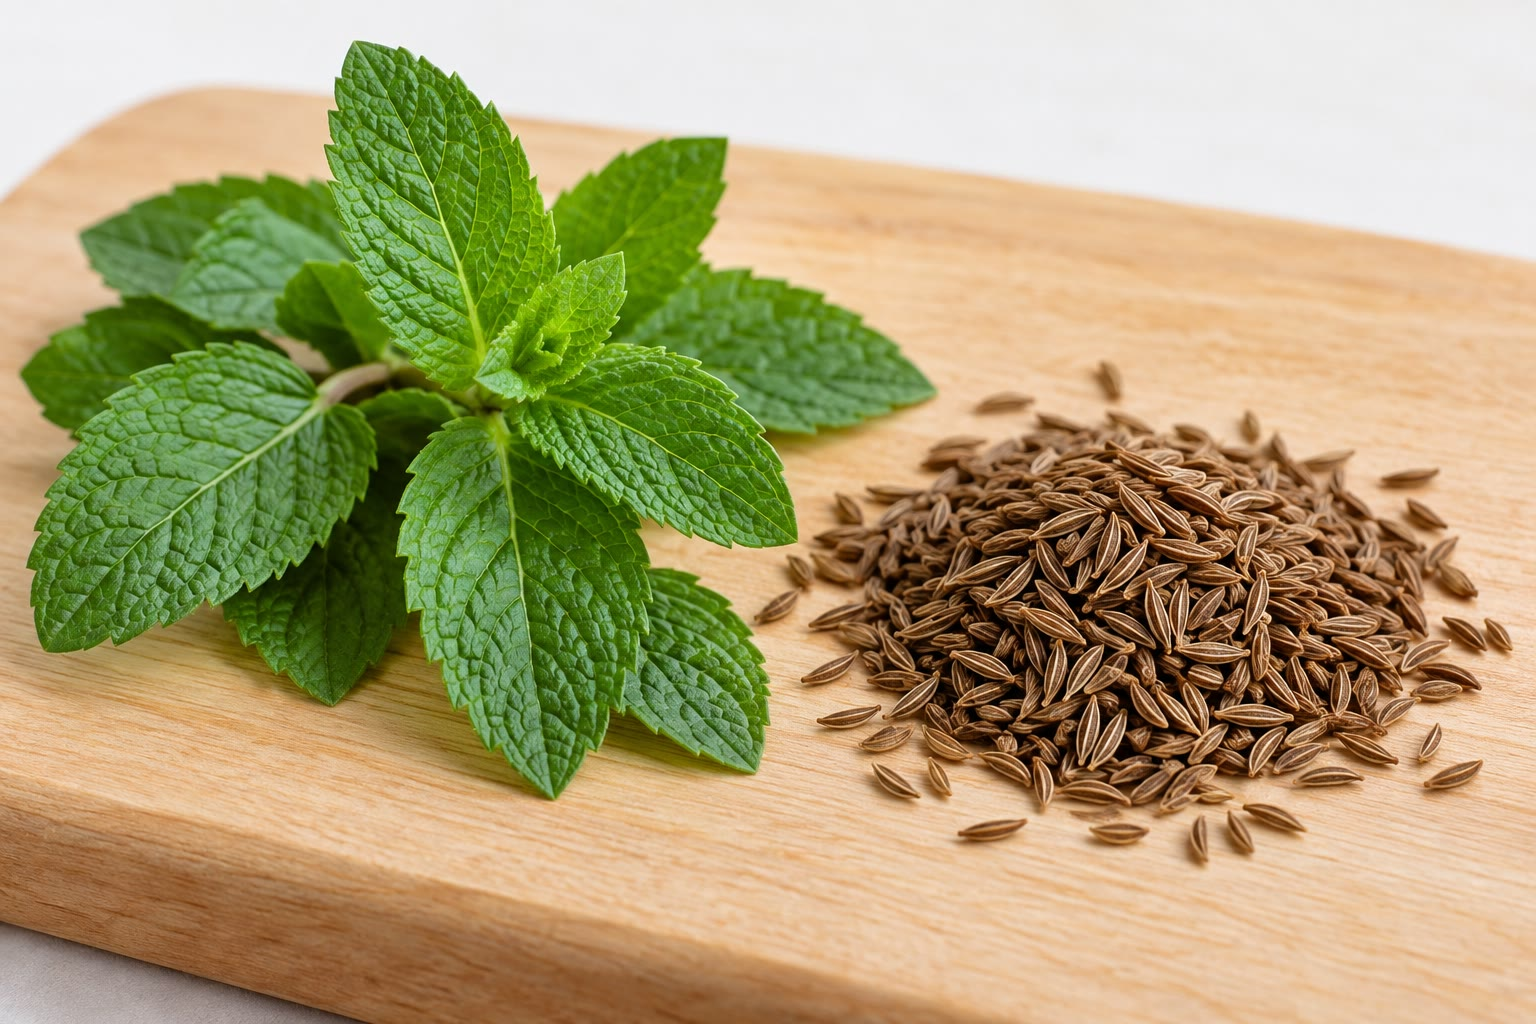
\includegraphics[width=0.48\linewidth]{images/book1/ai/g12-mint-caraway.jpg}

{\small Hierbabuena y alcaravea: dos \omterm{def:g7:atoms-and-molecules:molecule}{moléculas} especulares, dos olores.}
\end{omfigure}

\section{Las moléculas en el espacio}

\begin{definition}[Estereoisómeros]\label{def:g12:stereochemistry:stereoisomer}
Los \emph{estereoisómeros}\index{estereoisomeros@estereoisómeros} son \omterm{def:g7:atoms-and-molecules:molecule}{moléculas} con la
misma fórmula y la misma secuencia de \omterm{def:g7:atoms-and-molecules:atom}{átomos} enlazados, que solo se
diferencian por la disposición de sus \omterm{def:g7:atoms-and-molecules:atom}{átomos} en el espacio.
\end{definition}

\begin{definition}[Representación de Cram]\label{def:g12:stereochemistry:cram}
En la \emph{representación de Cram}\index{representacion de Cram@representación de Cram} de un
\omterm{def:g7:atoms-and-molecules:atom}{átomo} de carbono con cuatro enlaces simples, dos enlaces se dibujan en el
plano del papel como líneas normales, formando un ángulo; el enlace que
apunta hacia el lector, como una cuña llena, y el que se aleja, como una
cuña de trazos.
\end{definition}

\section{Quiralidad}

\begin{definition}[Quiral, carbono asimétrico]\label{def:g12:stereochemistry:chiral}
Un objeto o una \omterm{def:g7:atoms-and-molecules:molecule}{molécula} es \emph{quiral}\index{quiral} si no se puede
superponer a su imagen especular, como una mano. Un \omterm{def:g7:atoms-and-molecules:atom}{átomo} de carbono
unido a cuatro \omterm{def:g7:atoms-and-molecules:atom}{átomos} o grupos distintos es un \emph{carbono
asimétrico}\index{carbono asimetrico@carbono asimétrico}; a menudo se marca con un
asterisco.
\end{definition}

\begin{proposition}[Un carbono asimétrico hace quiral una molécula]\label{prop:g12:stereochemistry:one-carbon}
Una \omterm{def:g7:atoms-and-molecules:molecule}{molécula} con exactamente un \omterm{def:g12:stereochemistry:chiral}{carbono asimétrico} es \omterm{def:g12:stereochemistry:chiral}{quiral}.
\end{proposition}

\begin{proof}
Se admite: intercambiar dos de los cuatro grupos distintos que rodean al
\omterm{def:g12:stereochemistry:chiral}{carbono asimétrico} da la imagen especular, y ninguna rotación de la
\omterm{def:g7:atoms-and-molecules:molecule}{molécula} entera puede devolverla a la original, ya que los cuatro grupos
son todos distintos.
\end{proof}

\begin{definition}[Enantiómeros, mezcla racémica]\label{def:g12:stereochemistry:enantiomer}
Dos \omterm{def:g12:stereochemistry:stereoisomer}{estereoisómeros} que son imagen especular uno del otro y no son
superponibles son \emph{enantiómeros}\index{enantiomeros@enantiómeros}. Una \omterm{def:g6:pure-substances-and-mixtures:mixture}{mezcla} de
cantidades iguales de dos enantiómeros es una \emph{mezcla
racémica}\index{mezcla racemica@mezcla racémica}.
\end{definition}

\begin{omfigure}
\setchemfig{atom sep=2.2em}
\begin{tikzpicture}[font=\small]
  \node at (-2.4,0) {\chemfig{C(-[2]COOH)(-[4]H_3C)(<[:-30]OH)(<:[:-150]H)}};
  \node at (2.4,0) {\chemfig{C(-[2]COOH)(-[0]CH_3)(<[:-150]HO)(<:[:-30]H)}};
  \draw[dashed, omDef, thick] (0,-1.5) -- (0,1.6) node[above] {espejo};
  \node[anchor=north] at (-2.4,-1.4) {ácido láctico, A};
  \node[anchor=north] at (2.4,-1.4) {su imagen especular, B};
\end{tikzpicture}

{\small Los dos \omterm{def:g12:stereochemistry:enantiomer}{enantiómeros} del ácido láctico, \ce{CH3-CH(OH)-COOH}, en
\omterm{def:g12:stereochemistry:cram}{representación de Cram}. El carbono central es asimétrico (\ce{H}, \ce{OH},
\ce{CH3}, \ce{COOH}). Ninguna rotación convierte A en B: son tan distintos
como una mano izquierda y una derecha.}
\end{omfigure}

\begin{method}[¿Es quiral una molécula?]\label{met:g12:stereochemistry:chiral}
\begin{enumerate}
  \item Busca \omterm{def:g12:stereochemistry:chiral}{carbonos asimétricos}: un carbono con cuatro grupos
        distintos. Ninguno: la \omterm{def:g7:atoms-and-molecules:molecule}{molécula} (en este libro) no es \omterm{def:g12:stereochemistry:chiral}{quiral}.
  \item Exactamente uno: la \omterm{def:g7:atoms-and-molecules:molecule}{molécula} es \omterm{def:g12:stereochemistry:chiral}{quiral}.
  \item Dos o más: busca un plano que corte la \omterm{def:g7:atoms-and-molecules:molecule}{molécula} en dos mitades
        especulares, en alguna de sus formas; si existe, la \omterm{def:g7:atoms-and-molecules:molecule}{molécula} no
        es \omterm{def:g12:stereochemistry:chiral}{quiral}; si no, lo es.
\end{enumerate}
\end{method}

\begin{remark}[Mismas propiedades, olores distintos]\label{rem:g12:stereochemistry:same}
% ledger: smell:carvone-R, smell:carvone-S
Dos \omterm{def:g12:stereochemistry:enantiomer}{enantiómeros} tienen las mismas temperaturas de fusión y de
ebullición, la misma \omterm{def:g6:solutions-and-solubility:solubility}{solubilidad} y los mismos espectros: toda medida
hecha con algo que no es \omterm{def:g12:stereochemistry:chiral}{quiral} da el mismo resultado para ambos. Solo se
diferencian cuando se encuentran con algo \omterm{def:g12:stereochemistry:chiral}{quiral}, como la luz polarizada,
que desvían en sentidos opuestos, o los receptores de la nariz: una
carvona huele a hierbabuena y su \omterm{def:g12:stereochemistry:enantiomer}{enantiómero}, a alcaravea.
\end{remark}

\section{Diastereoisómeros}

\begin{definition}[Diastereoisómeros]\label{def:g12:stereochemistry:diastereomer}
Los \omterm{def:g12:stereochemistry:stereoisomer}{estereoisómeros} que no son imagen especular uno del otro son
\emph{diastereoisómeros}\index{diastereoisomeros@diastereoisómeros}. A diferencia de los
\omterm{def:g12:stereochemistry:enantiomer}{enantiómeros}, los diastereoisómeros tienen propiedades físicas distintas.
\end{definition}

\begin{proposition}[Contar estereoisómeros]\label{prop:g12:stereochemistry:count}
Una \omterm{def:g7:atoms-and-molecules:molecule}{molécula} con $n$ \omterm{def:g12:stereochemistry:chiral}{carbonos asimétricos} tiene como máximo $2^n$
\omterm{def:g12:stereochemistry:stereoisomer}{estereoisómeros}. Tiene menos cuando la \omterm{def:g7:atoms-and-molecules:molecule}{molécula} tiene dos mitades
iguales: entonces una de las combinaciones tiene un plano de simetría y
no es \omterm{def:g12:stereochemistry:chiral}{quiral} (una forma \emph{meso}).
\end{proposition}

\begin{proof}
Cada \omterm{def:g12:stereochemistry:chiral}{carbono asimétrico} puede adoptar dos disposiciones,
independientemente de los demás: $2 \times 2 \times \dots \times 2 = 2^n$ combinaciones. Cuando dos
combinaciones son la misma \omterm{def:g7:atoms-and-molecules:molecule}{molécula}, el recuento disminuye.
\end{proof}

\begin{omfigure}
\setchemfig{atom sep=1.9em}
\begin{tabular}{ccc}
\chemfig{HOOC-[:-30]C(<[:-90]OH)-[:30]C(<[:90]OH)-[:-30]COOH} &
\chemfig{HOOC-[:-30]C(<:[:-90]OH)-[:30]C(<:[:90]OH)-[:-30]COOH} &
\chemfig{HOOC-[:-30]C(<[:-90]OH)-[:30]C(<:[:90]OH)-[:-30]COOH} \\[4pt]
\small ácido L-tartárico & \small ácido D-tartárico & \small ácido meso-tartárico \\
\small (\omterm{def:g12:stereochemistry:chiral}{quiral}) & \small (\omterm{def:g12:stereochemistry:chiral}{quiral}, imagen especular del L) & \small (no \omterm{def:g12:stereochemistry:chiral}{quiral})
\end{tabular}

{\small Los tres \omterm{def:g12:stereochemistry:stereoisomer}{estereoisómeros} del ácido tartárico. L y D son
\omterm{def:g12:stereochemistry:enantiomer}{enantiómeros}; cada uno es \omterm{def:g12:stereochemistry:diastereomer}{diastereoisómero} de la forma meso, que tiene
un plano de simetría en una de sus formas: tres \omterm{def:g12:stereochemistry:stereoisomer}{estereoisómeros}, no
$2^2 = 4$.}
\end{omfigure}

\begin{history}[Pasteur separa cristales a mano, 1848]
En 1848, el joven químico Louis Pasteur observó con una lupa cristales
de una sal del ``ácido racémico'', una forma del ácido tartárico que no
desviaba la luz polarizada en ningún sentido. Se dio cuenta de que los
cristales tenían dos formas, cada una imagen especular de la otra, y los
separó uno a uno con unas pinzas. Una vez disueltos, un montón desviaba
la luz polarizada hacia la derecha y el otro, en la misma medida, hacia
la izquierda: el ácido racémico era una \omterm{def:g6:pure-substances-and-mixtures:mixture}{mezcla} de dos \omterm{def:g7:atoms-and-molecules:molecule}{moléculas}
especulares. Las \omterm{def:g7:atoms-and-molecules:molecule}{moléculas}, concluyó, pueden tener ``mano''.
\end{history}

\begin{omfigure}
\begin{minipage}[t]{0.36\linewidth}\centering
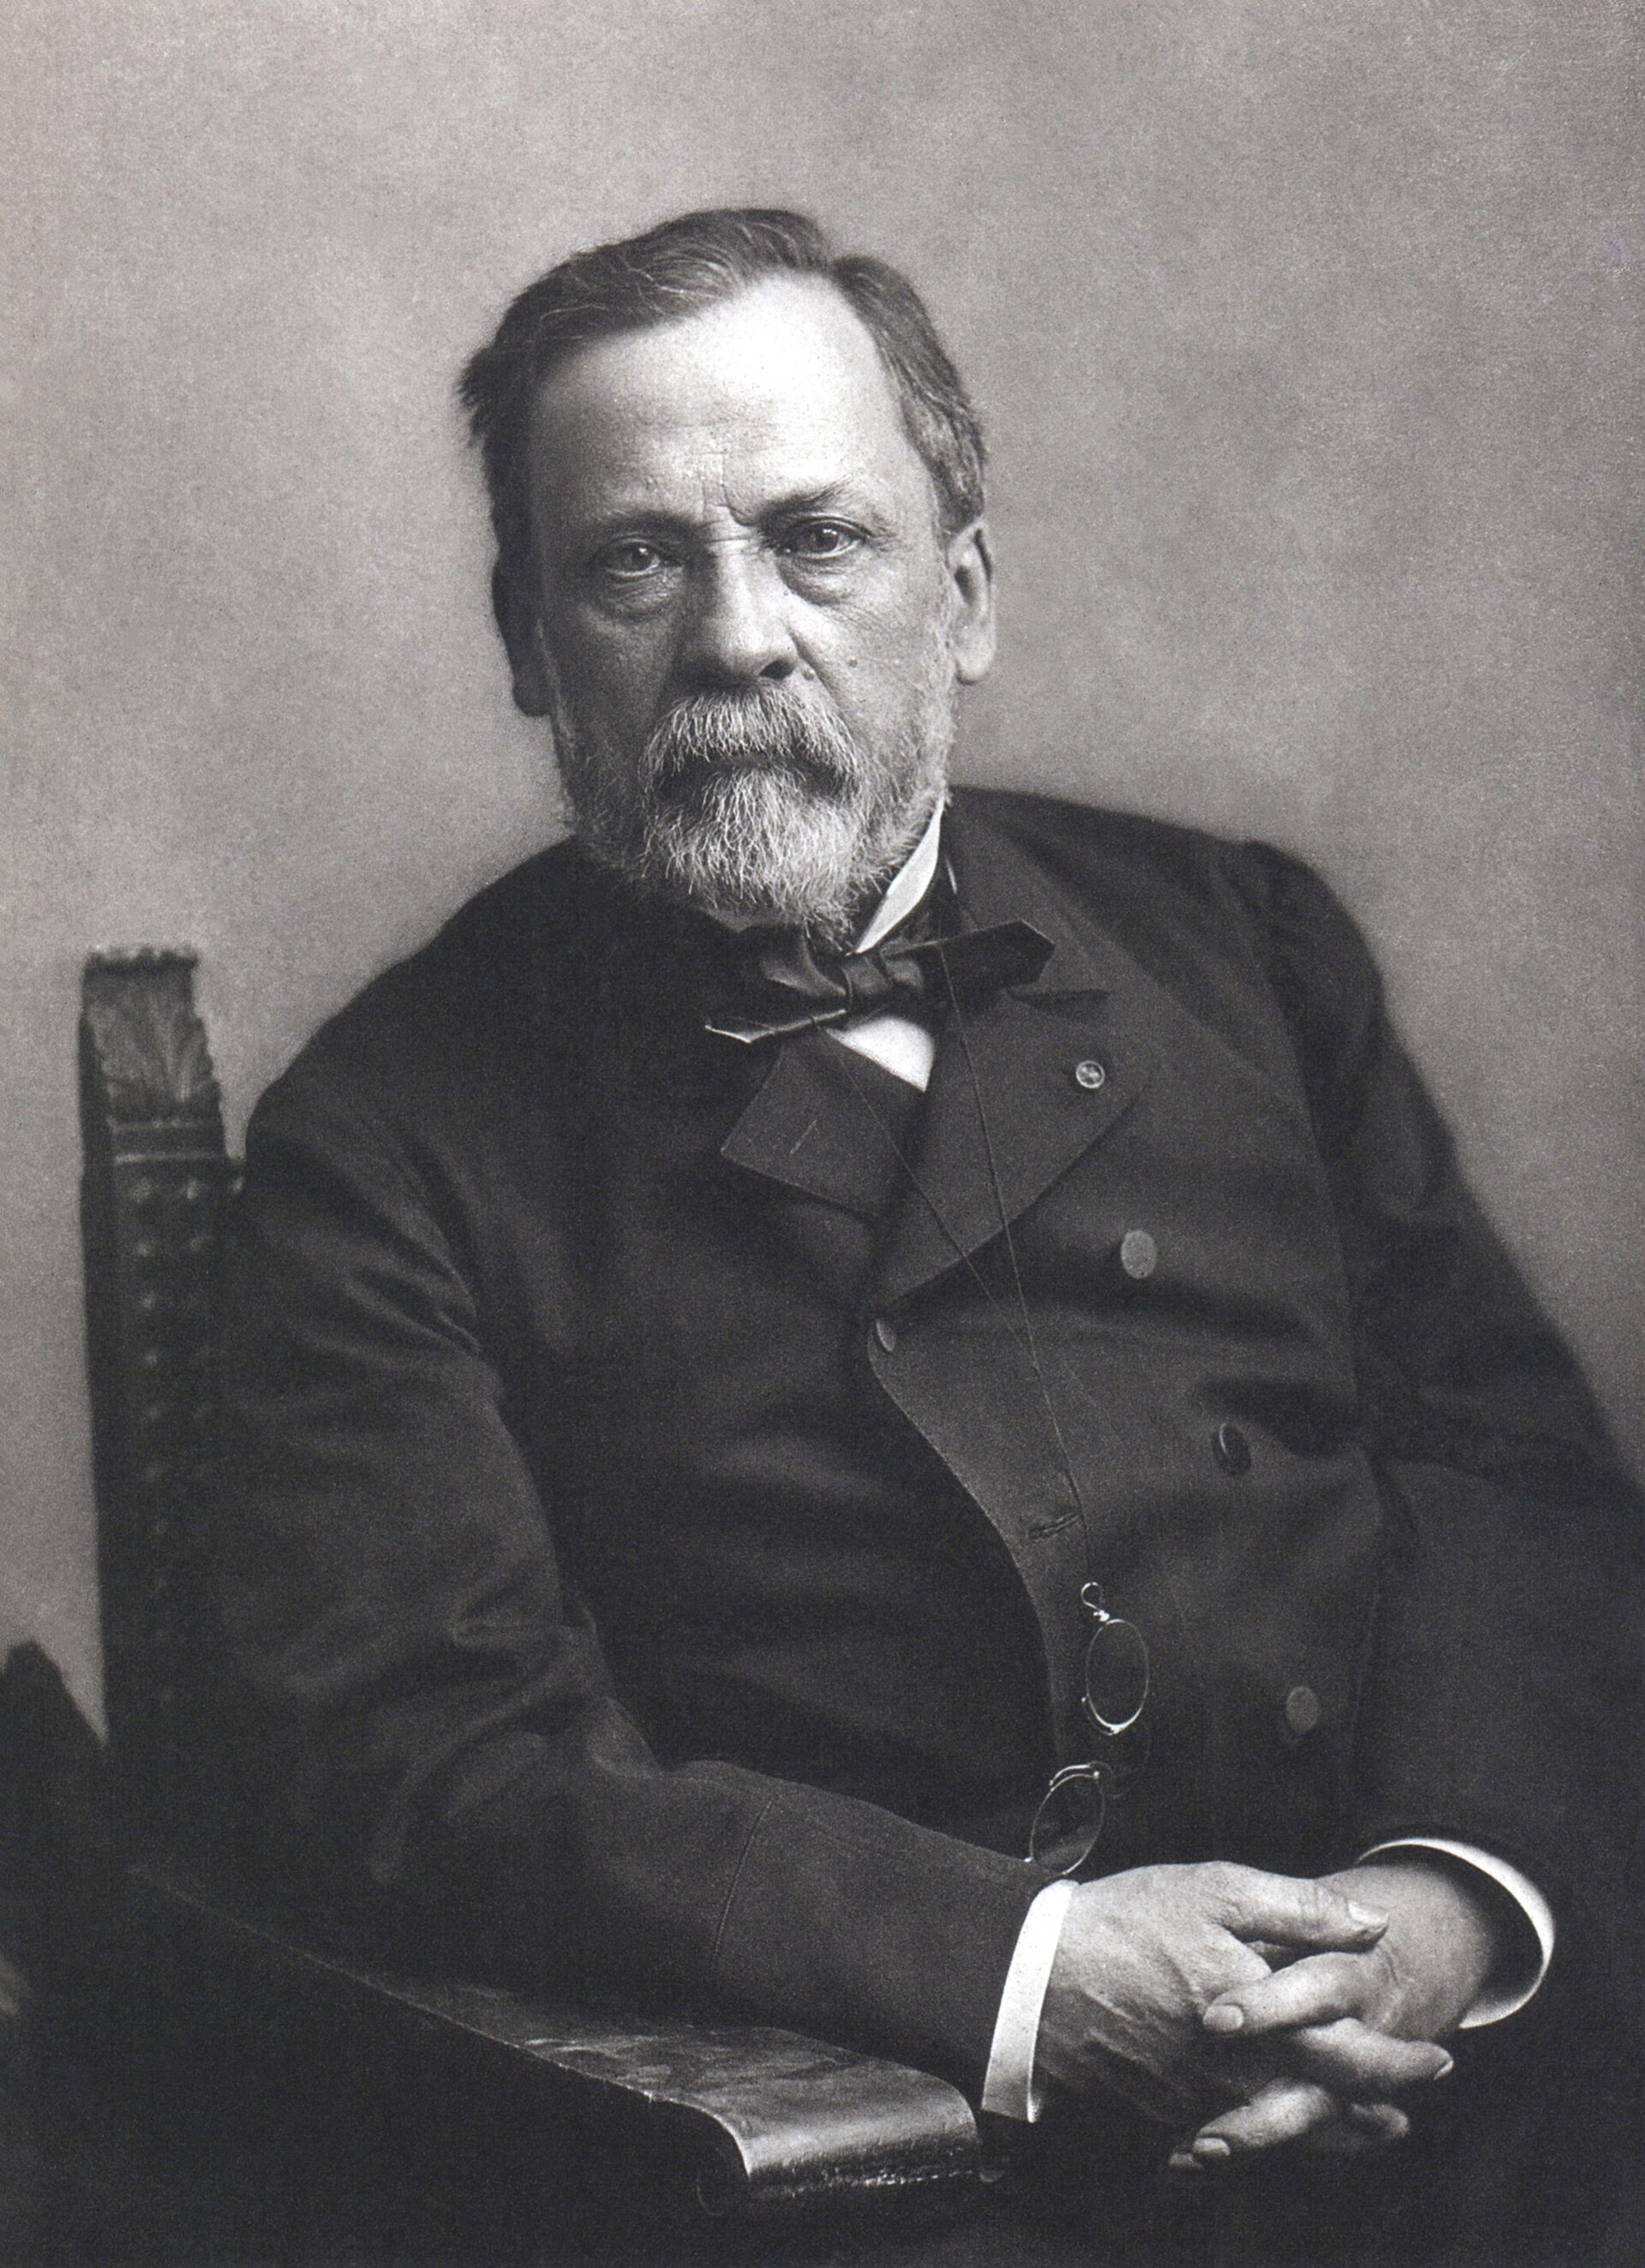
\includegraphics[height=5cm]{images/book1/pasteur.jpg}

{\small Louis Pasteur (1822--1895), fotografiado por Paul Nadar.}
\end{minipage}\qquad
\begin{minipage}[t]{0.36\linewidth}\centering
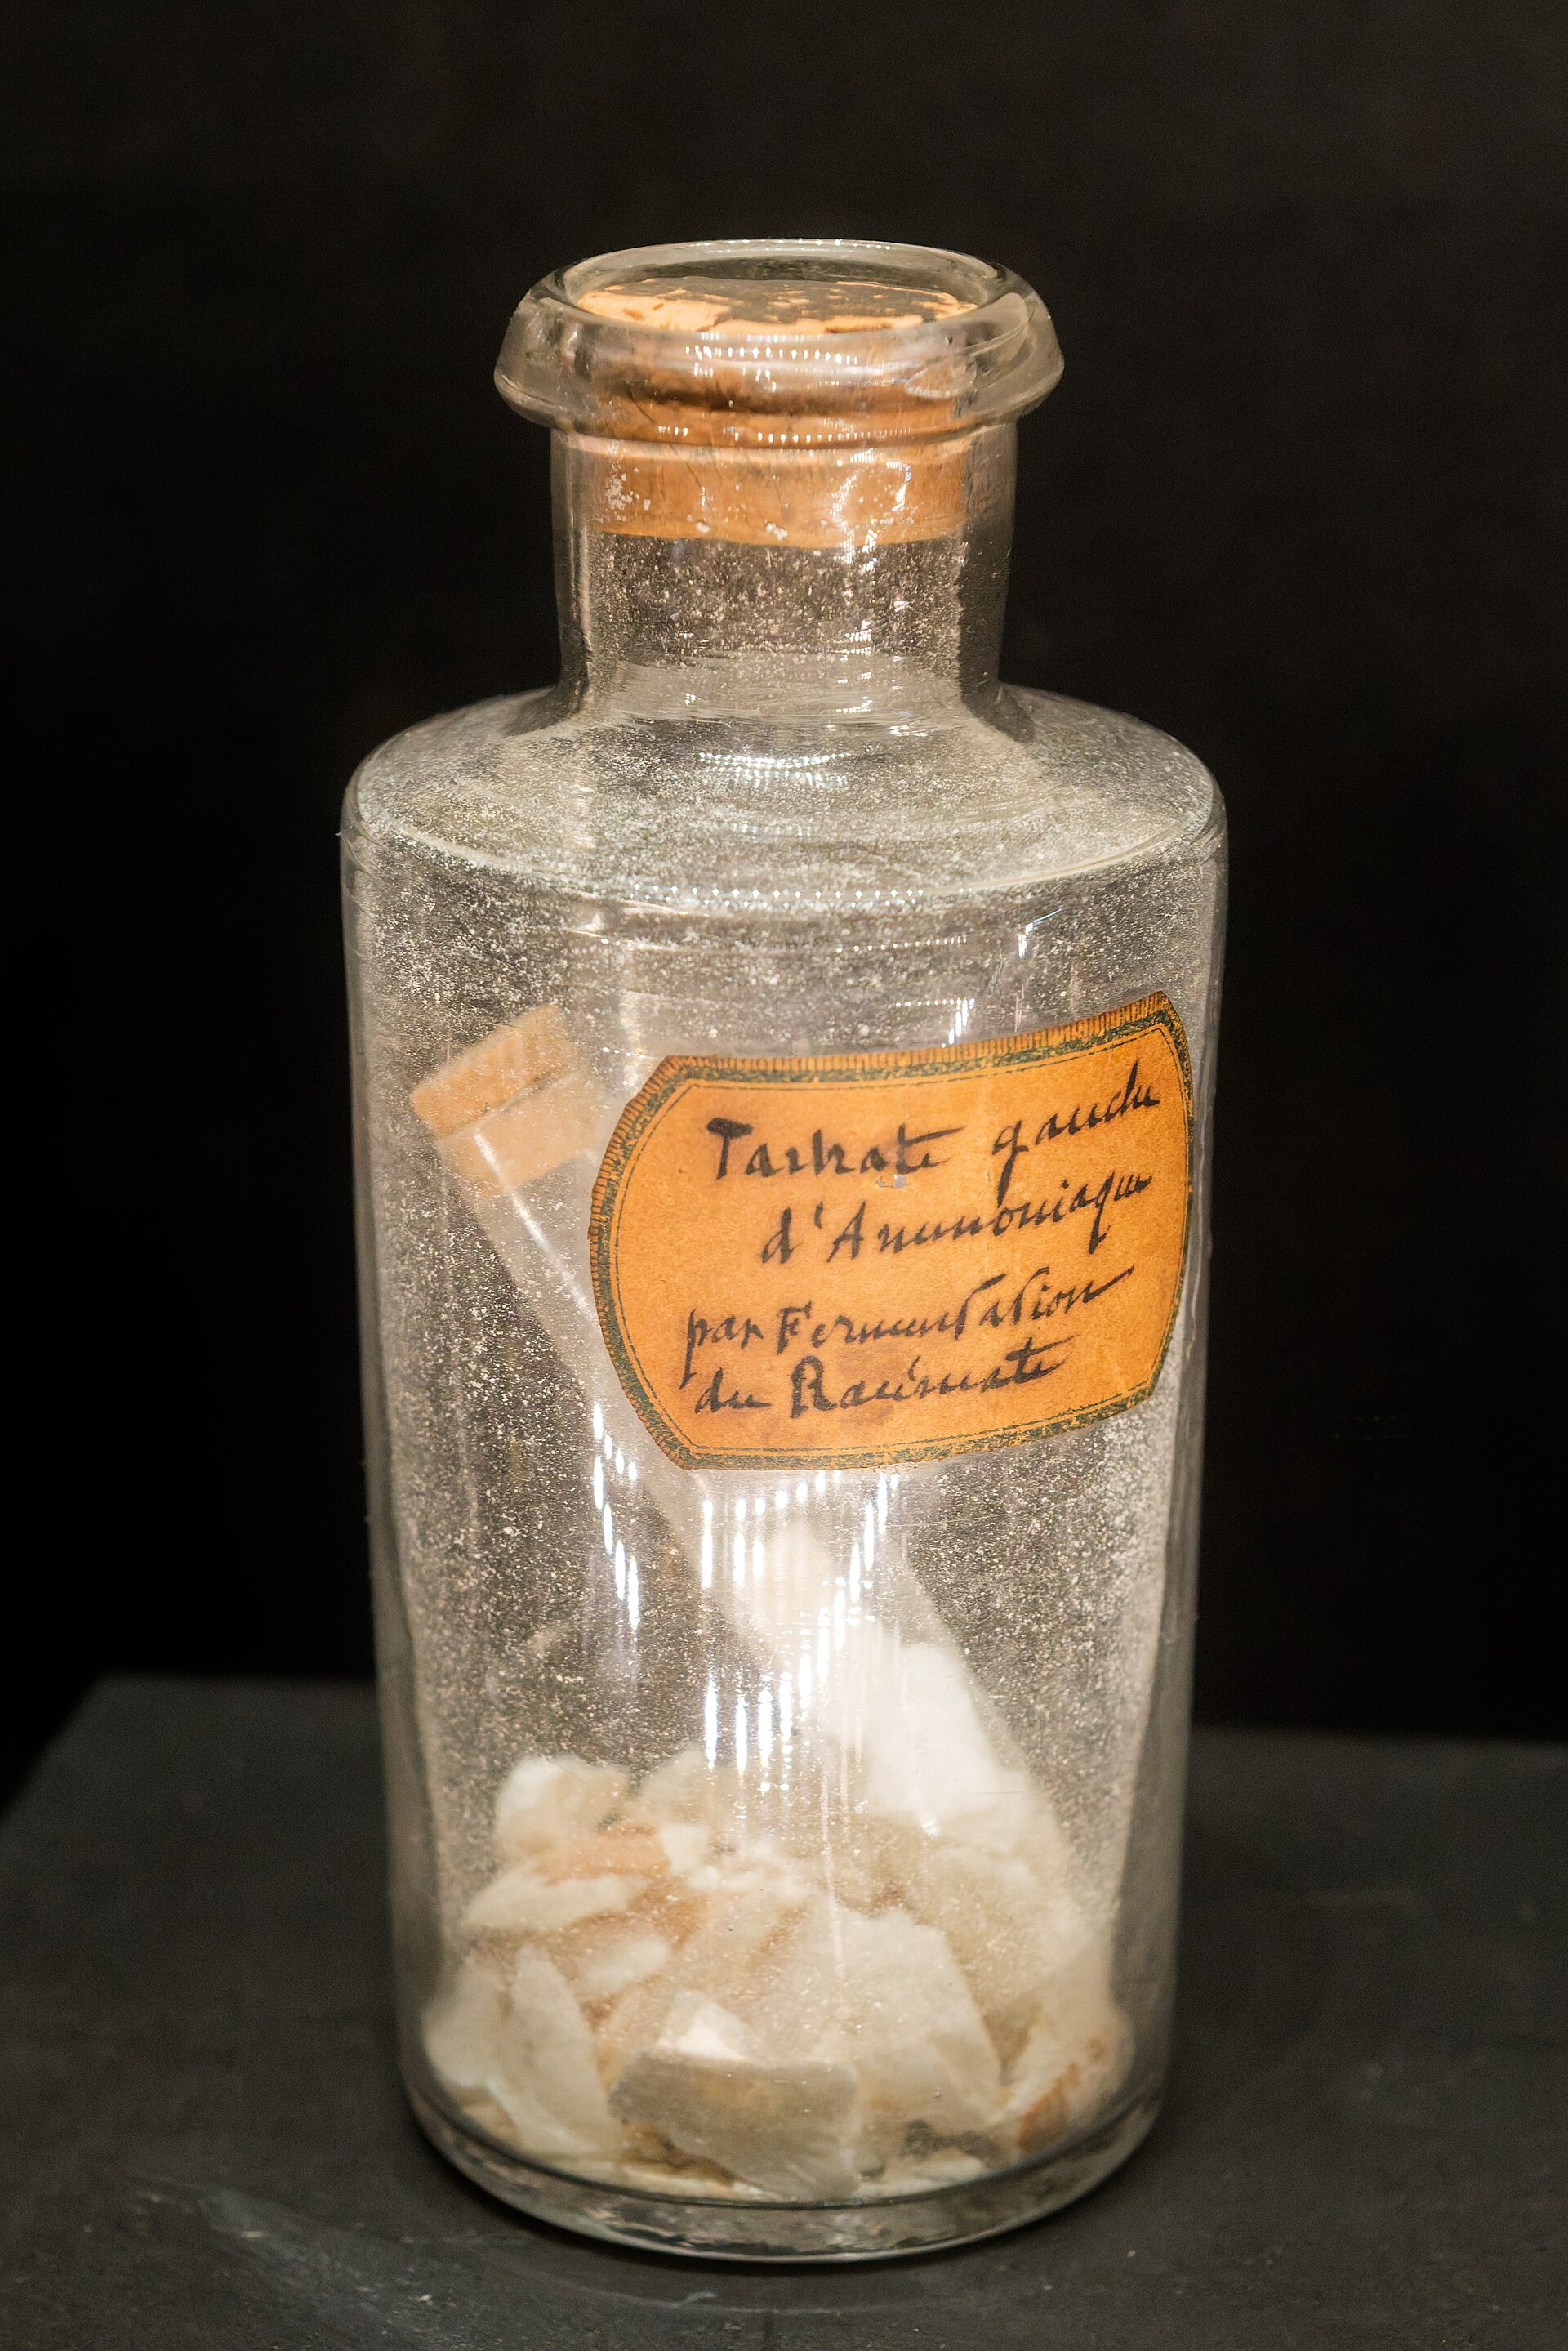
\includegraphics[height=5cm]{images/book1/tartrate-crystals.jpg}

{\small Cristales de tartrato de amonio de la colección de Pasteur. Foto
de Marie-Lan Taÿ Pamart, CC BY 4.0.}
\end{minipage}
\end{omfigure}

\section{Isómeros Z y E}


\begin{definition}[Isómeros Z y E]\label{def:g12:stereochemistry:z-e}
Cuando cada carbono de un \omterm{def:g10:lewis-and-shape:multiple-bond}{doble enlace} \ce{C=C} lleva dos \omterm{def:g7:atoms-and-molecules:atom}{átomos} o grupos
distintos, existen dos \omterm{def:g12:stereochemistry:stereoisomer}{estereoisómeros}, porque el \omterm{def:g10:lewis-and-shape:multiple-bond}{doble enlace} no gira.
En cada carbono tiene prioridad el grupo cuyo \omterm{def:g7:atoms-and-molecules:atom}{átomo} unido a él tiene el
mayor \omterm{def:g9:inside-the-atom:atomic-number}{número atómico}. Si los dos grupos prioritarios están del mismo lado
del \omterm{def:g10:lewis-and-shape:multiple-bond}{doble enlace}, el \omterm{def:g11:organic-skeletons:isomer}{isómero} es \emph{Z}\index{isomero Z@isómero Z}; si están en
lados opuestos, es \emph{E}\index{isomero E@isómero E}.
\end{definition}

\begin{method}[¿Z o E?]\label{met:g12:stereochemistry:z-e}
\begin{enumerate}
  \item Comprueba que cada carbono del \omterm{def:g10:lewis-and-shape:multiple-bond}{doble enlace} lleva dos grupos
        distintos; si no, no hay isomería \omterm{def:g12:stereochemistry:z-e}{Z}/\omterm{def:g12:stereochemistry:z-e}{E}.
  \item En cada carbono, da prioridad al grupo cuyo primer \omterm{def:g7:atoms-and-molecules:atom}{átomo} tiene el
        mayor \omterm{def:g9:inside-the-atom:atomic-number}{número atómico} (las reglas completas para los empates se
        dan en el volumen del primer año).
  \item Mismo lado: \omterm{def:g12:stereochemistry:z-e}{Z}. Lados opuestos: \omterm{def:g12:stereochemistry:z-e}{E}.
\end{enumerate}
\end{method}

\begin{omfigure}
\setchemfig{atom sep=2em}
\begin{tabular}{cc}
\chemfig{C(-[:150]H_3C)(-[:210]H)=C(-[:30]CH_3)(-[:-30]H)} &
\chemfig{C(-[:150]H_3C)(-[:210]H)=C(-[:30]H)(-[:-30]CH_3)} \\[4pt]
\small (\omterm{def:g12:stereochemistry:z-e}{Z})-but-2-eno: grupos \ce{CH3} del mismo lado &
\small (\omterm{def:g12:stereochemistry:z-e}{E})-but-2-eno: grupos \ce{CH3} en lados opuestos
\end{tabular}

{\small Los dos \omterm{def:g12:stereochemistry:stereoisomer}{estereoisómeros} del but-2-eno. En cada carbono, el
\ce{CH3} (carbono, $Z = 6$) tiene prioridad sobre el \ce{H} ($Z = 1$).
Son \omterm{def:g12:stereochemistry:diastereomer}{diastereoisómeros}: hierven a temperaturas distintas.}
\end{omfigure}

\section{Conformaciones}

\begin{definition}[Conformación]\label{def:g12:stereochemistry:conformation}
Los \omterm{def:g7:atoms-and-molecules:atom}{átomos} de una \omterm{def:g7:atoms-and-molecules:molecule}{molécula} pueden girar en torno a un enlace simple. Cada
disposición alcanzada mediante esos giros es una
\emph{conformación}\index{conformacion@conformación} de la \omterm{def:g7:atoms-and-molecules:molecule}{molécula}. Las
conformaciones de una misma \omterm{def:g7:atoms-and-molecules:molecule}{molécula} no son \omterm{def:g11:organic-skeletons:isomer}{isómeros}: se transforman
unas en otras continuamente a temperatura ambiente.
\end{definition}

\begin{omfigure}
\begin{tikzpicture}[font=\small]
  \pic (s) at (0,0) {omnewman={90}{30}};
  \foreach \k in {1,2,3} { \node at (s-f\k) {H}; \node at (s-b\k) {H}; }
  \node[anchor=north, align=center] at (0,-1.7) {alternada: los átomos H\\ de los dos carbonos se alternan};
  \pic (e) at (5,0) {omnewman={90}{112}};
  \foreach \k in {1,2,3} { \node at (e-f\k) {H}; \node[black!60] at (e-b\k) {H}; }
  \node[anchor=north, align=center] at (5,-1.7) {eclipsada: están enfrentados\\ (dibujados algo separados)};
\end{tikzpicture}

{\small Dos \omterm{def:g12:stereochemistry:conformation}{conformaciones} del etano, \ce{CH3-CH3}, vistas a lo largo del
enlace \ce{C-C}: el carbono delantero es el centro y el trasero, el
círculo. La \omterm{def:g12:stereochemistry:conformation}{conformación} alternada, en la que los \omterm{def:g7:atoms-and-molecules:atom}{átomos} están lo más
alejados posible, es la más estable.}
\end{omfigure}

\begin{remark}[Por qué importa]\label{rem:g12:stereochemistry:matters}
Los seres vivos están formados por \omterm{def:g7:atoms-and-molecules:molecule}{moléculas} \omterm{def:g12:stereochemistry:chiral}{quirales} (proteínas,
azúcares), y los receptores y las enzimas hechos de ellas distinguen los
\omterm{def:g12:stereochemistry:enantiomer}{enantiómeros}: dos \omterm{def:g12:stereochemistry:enantiomer}{enantiómeros} pueden oler, saber o actuar como
medicamentos de forma muy distinta. Por eso los químicos que fabrican un
fármaco con un \omterm{def:g12:stereochemistry:chiral}{carbono asimétrico} deben saber qué \omterm{def:g12:stereochemistry:enantiomer}{enantiómero} obtienen, y
ensayar cada uno.
\end{remark}

\section{Ejercicios}

\begin{exercise}[$\star$]\label{exo:g12:stereochemistry:1}
¿Cuáles de estas \omterm{def:g7:atoms-and-molecules:molecule}{moléculas} tienen un \omterm{def:g12:stereochemistry:chiral}{carbono asimétrico}? Márcalo con un
asterisco. Butan-2-ol \ce{CH3-CH(OH)-CH2-CH3}; propan-2-ol
\ce{CH3-CH(OH)-CH3}; 2-clorobutano; ácido láctico \ce{CH3-CH(OH)-COOH}.
\end{exercise}

\begin{exercise}[$\star$]\label{exo:g12:stereochemistry:2}
¿Es cada \omterm{def:g12:stereochemistry:z-e}{isómero Z} o \omterm{def:g12:stereochemistry:z-e}{E}?
\begin{center}
\setchemfig{atom sep=1.8em}
\chemfig{C(-[:150]Cl)(-[:210]H)=C(-[:30]Cl)(-[:-30]H)} \qquad
\chemfig{C(-[:150]H_3C)(-[:210]H)=C(-[:30]H)(-[:-30]CH_2-CH_3)}
\end{center}
\end{exercise}

\begin{exercise}[$\star$]\label{exo:g12:stereochemistry:3}
¿Cuáles son \omterm{def:g12:stereochemistry:chiral}{quirales}: un guante, una cuchara, un tornillo, un cubo? ¿Cuál
de las \omterm{def:g7:atoms-and-molecules:molecule}{moléculas} \ce{CH2Cl2} y \ce{CHFClBr} es \omterm{def:g12:stereochemistry:chiral}{quiral}?
\end{exercise}

\begin{exercise}[$\star$]\label{exo:g12:stereochemistry:4}
¿Qué es una \omterm{def:g12:stereochemistry:enantiomer}{mezcla racémica}? En el caso de la carvona, ¿huele a
hierbabuena, a alcaravea o a ambas?
\end{exercise}

\begin{exercise}[$\star$]\label{exo:g12:stereochemistry:5}
¿Puede el but-1-eno \ce{CH2=CH-CH2-CH3} existir como \omterm{def:g12:stereochemistry:z-e}{isómeros Z} y \omterm{def:g12:stereochemistry:z-e}{E}?
¿Por qué?
\end{exercise}

\begin{exercise}[$\star\star$]\label{exo:g12:stereochemistry:6}
Dibuja los dos \omterm{def:g12:stereochemistry:enantiomer}{enantiómeros} del butan-2-ol en \omterm{def:g12:stereochemistry:cram}{representación de Cram}, con
un espejo entre ellos.
\end{exercise}

\begin{exercise}[$\star\star$]\label{exo:g12:stereochemistry:7}
¿Cuántos \omterm{def:g12:stereochemistry:stereoisomer}{estereoisómeros} tienen: el 2-clorobutano; el
2,3-diclorobutano \ce{CH3-CHCl-CHCl-CH3}; el pent-2-eno
\ce{CH3-CH=CH-CH2-CH3}?
\end{exercise}

\begin{exercise}[$\star\star$]\label{exo:g12:stereochemistry:8}
Di si estas parejas son \omterm{def:g12:stereochemistry:enantiomer}{enantiómeros}, \omterm{def:g12:stereochemistry:diastereomer}{diastereoisómeros} o la misma
\omterm{def:g7:atoms-and-molecules:molecule}{molécula}: ácido L- y D-tartárico; ácido L- y meso-tartárico; (\omterm{def:g12:stereochemistry:z-e}{Z})- y
(\omterm{def:g12:stereochemistry:z-e}{E})-but-2-eno; ácido meso-tartárico y su propia imagen especular.
\end{exercise}

\begin{exercise}[$\star\star$]\label{exo:g12:stereochemistry:9}
El butano, \ce{CH3-CH2-CH2-CH3}, visto a lo largo de su enlace central.
Dibuja la \omterm{def:g12:stereochemistry:conformation}{conformación} alternada en la que los dos grupos \ce{CH3} están
opuestos, y una eclipsada en la que están enfrentados. ¿Cuál es la más
estable? ¿Por qué?
\end{exercise}

\begin{exercise}[$\star\star$]\label{exo:g12:stereochemistry:10}
El ácido meso-tartárico tiene dos \omterm{def:g12:stereochemistry:chiral}{carbonos asimétricos}, pero no es
\omterm{def:g12:stereochemistry:chiral}{quiral}. Explícalo usando su plano de simetría.
\end{exercise}

\begin{exercise}[$\star\star$]\label{exo:g12:stereochemistry:11}
Dibuja y nombra los \omterm{def:g12:stereochemistry:z-e}{isómeros Z} y \omterm{def:g12:stereochemistry:z-e}{E} del pent-2-eno.
\end{exercise}

\begin{exercise}[$\star\star\star$]\label{exo:g12:stereochemistry:12}
El 2,3-dibromobutano \ce{CH3-CHBr-CHBr-CH3} tiene dos \omterm{def:g12:stereochemistry:chiral}{carbonos
asimétricos}. Dibuja sus \omterm{def:g12:stereochemistry:stereoisomer}{estereoisómeros} en la representación en zigzag
usada para el ácido tartárico, y demuestra que uno de ellos es una forma
meso.
\end{exercise}

\begin{exercise}[$\star\star\star$]\label{exo:g12:stereochemistry:13}
Una \omterm{def:g7:atoms-and-molecules:molecule}{molécula} de un fármaco tiene un \omterm{def:g12:stereochemistry:chiral}{carbono asimétrico}. Su \omterm{def:g10:synthesis-yield:synthesis}{síntesis} da
una \omterm{def:g12:stereochemistry:enantiomer}{mezcla racémica}, pero solo un \omterm{def:g12:stereochemistry:enantiomer}{enantiómero} encaja en el receptor
\omterm{def:g12:stereochemistry:chiral}{quiral} sobre el que debe actuar. ¿Qué fracción del medicamento racémico
es activa? Indica dos maneras en que un químico podría hacerlo mejor.
\end{exercise}

\begin{exercise}[$\star\star\star$]\label{exo:g12:stereochemistry:14}
El hexa-2,4-dieno, \ce{CH3-CH=CH-CH=CH-CH3}, tiene dos \omterm{def:g10:lewis-and-shape:multiple-bond}{dobles enlaces}, y
cada uno puede ser \omterm{def:g12:stereochemistry:z-e}{Z} o \omterm{def:g12:stereochemistry:z-e}{E}. ¿Cuántos \omterm{def:g12:stereochemistry:stereoisomer}{estereoisómeros} tiene? (Cuidado con
la simetría de la \omterm{def:g7:atoms-and-molecules:molecule}{molécula}.)
\end{exercise}

\begin{exercise}[$\star\star\star$]\label{exo:g12:stereochemistry:15}
Una \omterm{def:g7:atoms-and-molecules:molecule}{molécula} de azúcar tiene tres \omterm{def:g12:stereochemistry:chiral}{carbonos asimétricos} y ninguna
simetría. ¿Cuántos \omterm{def:g12:stereochemistry:stereoisomer}{estereoisómeros} puede tener como máximo? ¿Cuántas
parejas de \omterm{def:g12:stereochemistry:enantiomer}{enantiómeros} representa eso? ¿Cuántos \omterm{def:g12:stereochemistry:diastereomer}{diastereoisómeros}
tiene cada \omterm{def:g12:stereochemistry:stereoisomer}{estereoisómero}?
\end{exercise}

\section{Problema: los cristales de Pasteur}


\begin{problem}[{Problema de fin de semana --- el ácido tartárico tiene dos
carbonos asimétricos: ¿cuántos estereoisómeros tiene en realidad?}]
\label{pb:g12:stereochemistry:1}
% ledger: mp:tartaric-L, aw:C, aw:H, aw:O
Las formas del ácido tartárico, \ce{HOOC-CH(OH)-CH(OH)-COOH}, tuvieron
un papel decisivo en el descubrimiento de que las \omterm{def:g7:atoms-and-molecules:molecule}{moléculas} pueden tener
``mano''. El ácido L-tartárico funde hacia \qty{169}{\celsius}.

\medskip
\noindent\textbf{Parte I --- La \omterm{def:g7:atoms-and-molecules:molecule}{molécula}.}
\begin{enumerate}
  \item Da la \omterm{def:g11:organic-skeletons:formulas}{fórmula molecular} del ácido tartárico y su \omterm{def:g10:the-mole:molar-mass}{masa molar}.
  \item Nombra sus \omterm{def:g11:functional-groups:functional-group}{grupos funcionales} e indica cuántos hay de cada uno.
  \item ¿Qué \omterm{def:g7:atoms-and-molecules:atom}{átomos} de carbono son asimétricos? Enumera los cuatro grupos
        de cada uno.
  \item Según la regla de este capítulo, ¿cuántos \omterm{def:g12:stereochemistry:stereoisomer}{estereoisómeros} podría
        tener como máximo?
\end{enumerate}

\medskip
\noindent\textbf{Parte II --- Los \omterm{def:g12:stereochemistry:stereoisomer}{estereoisómeros}.}
\begin{enumerate}[resume]
  \item En el dibujo en zigzag del ácido L-tartárico, ¿los grupos
        \ce{OH} se dibujan con cuñas llenas o de trazos?
  \item Dibuja su imagen especular. ¿Se pueden superponer las dos?
        Nombra la imagen especular.
  \item Dibuja la forma con una cuña llena y una de trazos. Hazla girar
        mentalmente en torno al enlace central y encuentra un plano de
        simetría.
  \item ¿Es \omterm{def:g12:stereochemistry:chiral}{quiral} esta forma? ¿Cómo se llama?
  \item Explica por qué el ácido tartárico solo tiene tres
        \omterm{def:g12:stereochemistry:stereoisomer}{estereoisómeros}.
  \item Di si L y D, y luego L y meso, son \omterm{def:g12:stereochemistry:enantiomer}{enantiómeros} o
        \omterm{def:g12:stereochemistry:diastereomer}{diastereoisómeros}.
\end{enumerate}

\medskip
\noindent\textbf{Parte III --- Propiedades.}
\begin{enumerate}[resume]
  \item ¿A qué temperatura funde el ácido D-tartárico? ¿Por qué?
  \item ¿Tiene que fundir el ácido meso-tartárico a la misma temperatura?
        ¿Por qué?
  \item La carvona muestra que dos \omterm{def:g12:stereochemistry:enantiomer}{enantiómeros} pueden oler distinto.
        ¿Por qué una nariz puede distinguirlos y un termómetro no?
  \item Una \omterm{def:g12:stereochemistry:enantiomer}{mezcla racémica} de ácido L- y D-tartárico: ¿es una \omterm{def:g6:pure-substances-and-mixtures:pure-substance}{sustancia
        pura}? ¿Es ópticamente activa en conjunto?
\end{enumerate}

\medskip
\noindent\textbf{Parte IV --- Pasteur.}
\begin{enumerate}[resume]
  \item La sal racémica de Pasteur daba cristales de dos formas
        especulares. ¿Qué contenía cada cristal?
  \item A partir de \qty{10.0}{g} de sal racémica, ¿qué masa de cada tipo
        de cristal podía esperar?
  \item ¿Por qué la forma meso nunca aparece entre esos cristales?
  \item ¿Cómo podía comprobar, tras la separación, que los dos montones
        eran \omterm{def:g12:stereochemistry:enantiomer}{enantiómeros}?
  \item El 3-clorobutan-2-ol, \ce{CH3-CHCl-CH(OH)-CH3}, también tiene dos
        \omterm{def:g12:stereochemistry:chiral}{carbonos asimétricos}. ¿Cuántos \omterm{def:g12:stereochemistry:stereoisomer}{estereoisómeros} tiene? ¿Por qué no
        pierde uno como el ácido tartárico?
  \item Da la respuesta final: ¿cuántos \omterm{def:g12:stereochemistry:stereoisomer}{estereoisómeros} tiene el ácido
        tartárico?
\end{enumerate}
\end{problem}
